\documentclass{beamer}
\usepackage[utf8]{inputenc}
\usepackage[french]{babel}
\usepackage{graphics}
\usepackage{tabularx}
\usepackage[french]{babel}
\usepackage[T1]{fontenc}


%\usepackage[screen,nopanel]{pdfscreen}
%\usepackage{url}

\usetheme[progressbar=frametitle,numbering=none]{metropolis}
\definecolor{Pourpre}{RGB}{174,37,115} 
\setbeamercolor{alerted text}{fg=Pourpre}
%\setbeamertemplate{itemize items}{\textcolor{Pourpre}{\footnotesize$\blacksquare$}}

\title{Initiation et développement de l'agilité en DUT Informatique}
\author[Thomas Clavier, Yann Secq]
{
  \{ \textbf{Thomas.Clavier \& Yann.Secq} \}\texttt{@univ-lille1.fr}
}
\institute{
  
\includegraphics[height=13mm]{includes/logo_iut_A_Lille.jpg}
  
\includegraphics[height=13mm]{includes/logo_Univ_de_Lille.jpg}
}
  
\date{}

\logo{
    
\includegraphics[width=1cm]{includes/CC_BY_SA} 
}

\begin{document}

\frame{\titlepage}

\begin{frame}{Bipodocratie}
  \begin{columns}
    \begin{column}{0.5\textwidth}
      \begin{center}
        
\includegraphics[width=0.6\textwidth]{includes/foots.png}      
      \end{center}
    \end{column}
    \begin{column}{0.5\textwidth}
      Si vous n’apprenez rien ou que vous ne contribuez pas, passez à autre chose !
    \end{column}
  \end{columns}
\end{frame}

\section{Introduction}
\begin{frame}{Enseignement de l'agilité à l'Université}
Tribulations à l'Université d'un agiliste professionnel et de son compère enseignant-chercheur en quête d'une révolution de la pédagogie académique
   \begin{itemize}
     \item Pourquoi de l'agilité en DUT ?
     \item Comment tout a démarré
     \item Des petits pas
     \item Et maintenant ?
   \end{itemize}
\end{frame}

\begin{frame}{Pourquoi de l'agilité en DUT}
   \begin{itemize}
    \item DUT, une fabrique de développeurs
    \item Contact direct et (assez) étroit avec les réalités professionnelles
    \item Info: algorithmique et programmation, système et réseau, base de données, méthodologie et analyse
    \item Enseignement académique $\Rightarrow$ silos disciplinaires :(
    \item Réforme du PPN en 2013 $\Rightarrow$ projet de semestre
   \end{itemize}
\end{frame}

\begin{frame}{Comment tout a démarré}
   \begin{itemize}
     \item Un réseau national structuré ...
     \item Les <<grandes>> Journées Agiles(Toulouse'12, Aix'13, Montreuil'14)
     \item Les <<petites>> Journées Agiles (\textbf{Lille'13}, Lyon'14)
     \item Premier poste de PAST au département pour septembre 2013 !
     %\item Début des projets sur la lune pour Laurel et Hardy ;)
   \end{itemize}
\end{frame}

{
\usebackgroundtemplate{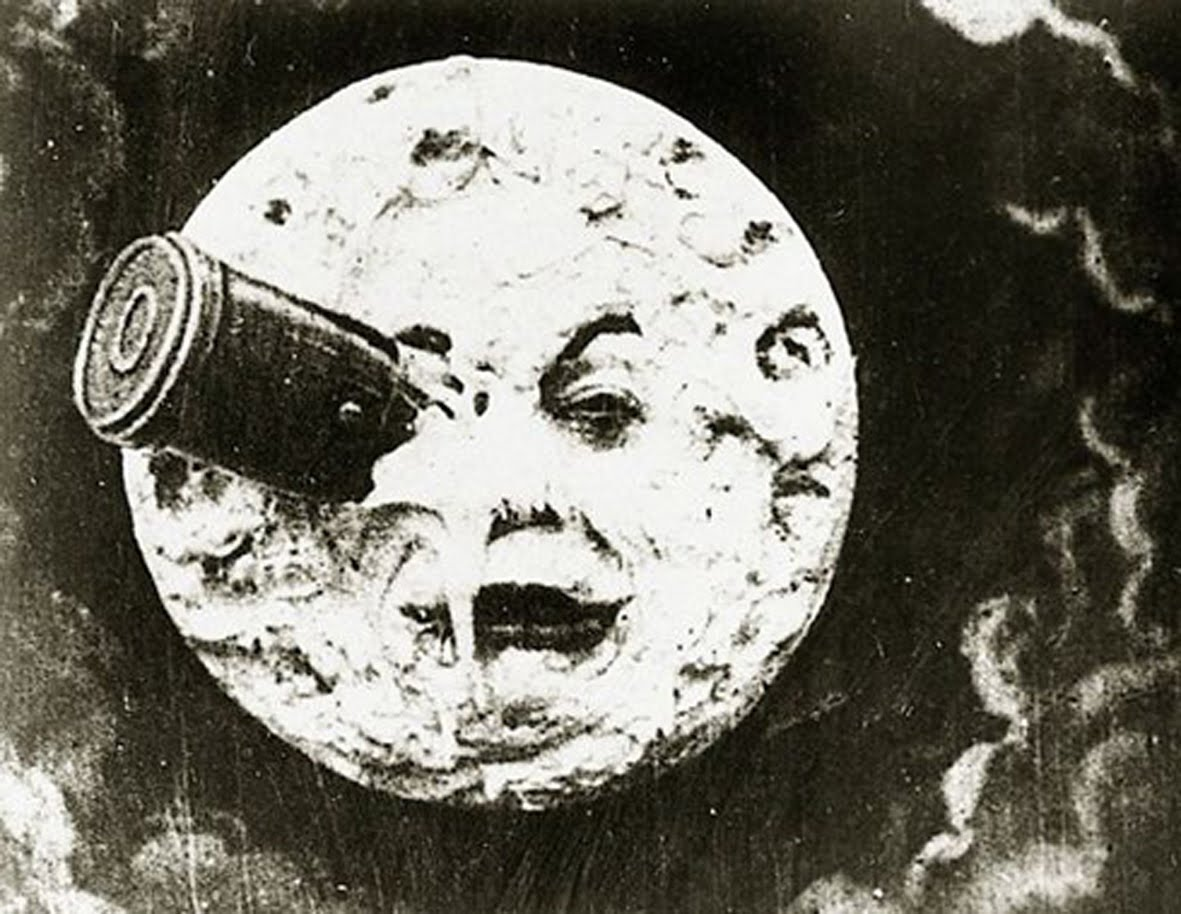
\includegraphics[width=\paperwidth]{includes/le-voyage-dans-la-lune-oeil.jpg}}
\begin{frame}[plain]
\end{frame}
}

\section{Janvier 2014}
\subsection{Objectifs}
\begin{frame}{Janvier 2014 : Expérience}
  Premier projet agile, un groupe de S3.

  Objectifs : 
  \begin{itemize}
    \item découvrir l'agilité et l'amélioration continue à travers un vrai projet : radiateur d'information, démo, rétro, PDCA
    \item prototyper rapidement un produit web avec un serveur REST du JS, html et bootstrap.
    \item prouver aux collègues que c'est possible pour le passer à plus grande échelle. 
  \end{itemize}
\end{frame}

\subsection{Deroulement}
\begin{frame}{Janvier 2014 : Déroulement}
  \begin{itemize}
    \item 2 encadrants pour un groupe de TP (26 étudiants).
    \item les étudiants s'organisent entre eux pour faire des équipes de 6 ou 7.
    \item des sujets apportés par les étudiants
    \item des contraintes technique forte
  \end{itemize}
\end{frame}

\begin{frame}{Janvier 2014 : Planning}
  \begin{center}
    \begin{tabular}{| c | c | c |}
      \hline
      \textbf{Jour 1} & \textbf{Jour 2} & \textbf{Jour 3} \\
      \hline \hline
      Lego4scrum & sprint & sprint \\
      \hline
      backlog & sprint & sprint \\
      \hline \hline
      sprint 0 & sprint & soutenance \\
      \hline
      sprint & sprint & rétrospective \\
      \hline
    \end{tabular}
  \end{center}
\end{frame}

\subsection{Apprentissages}
\begin{frame}{Janvier 2014 : Apprentissages}
  \begin{itemize}
    \item 1 enseignant pour 13 étudiants c'est très bien,
    \item la généralisation à toute la promo est possible
    \item plonger les étudiants dans un contexte technique innovant avec une bonne base théorique (ie. en fin d'IUT) c'est déstabilisant et très formateur. 
    \item activité trop courte pour à la foi faire le backlog, le découper et le coder.
  \end{itemize}
\end{frame}

%\begin{frame}{Année 1 (septembre 2013 à juillet 2014)}
%  \begin{itemize}
%    \item de 96h théoriques à XXh pour l'agilité ...
%    \item \textbf{Problématique:} \emph{proof of concept}
%    \item première expérimentation: à petite échelle
%        \begin{itemize}
%          \item le groupe "PE" de 26 étudiants
%          \item constitution des équipes par les enseignants
%          \item 3 jours entre le S3 et le S4 (impact collègues)
%          \item sprint de 1h30 + 15mn démo + 15mn rétro
%          \item restitution et démo finale \emph{(plus sûr de ça !)}
%          \item rétrospective \textbf{très} enthousiaste des étudiants :)
%        \end{itemize}
%    \item \textbf{Objectif n+1}: généralisation à toute la promotion de S3 !
%  \end{itemize}
%\end{frame}

\section{Octobre 2014}
\subsection{Objectifs}
\begin{frame}{Octobre 2014 : Objectifs}
  \begin{columns}
    \begin{column}{0.5\textwidth}
      \begin{center}
        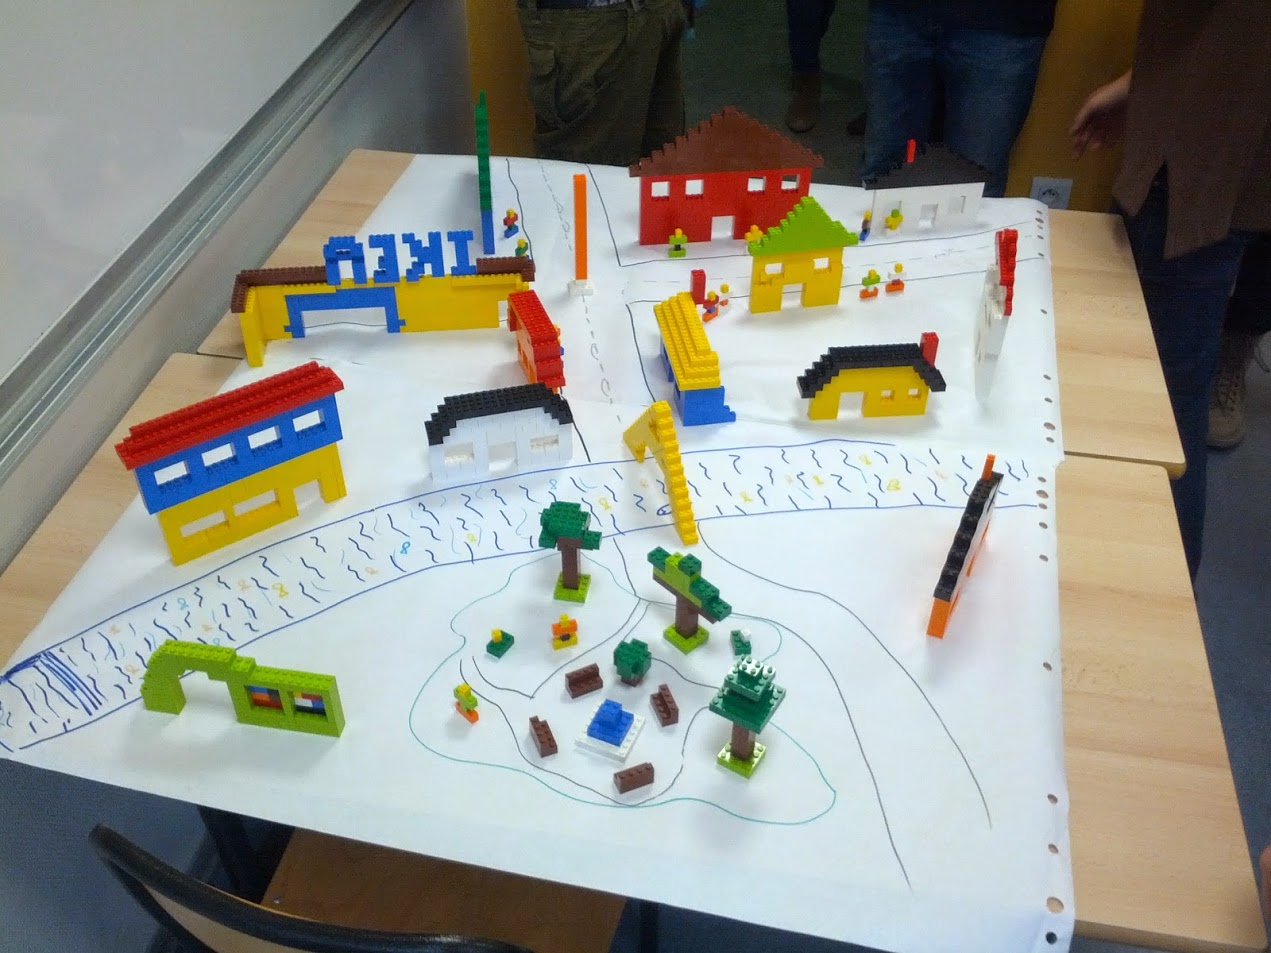
\includegraphics[width=\textwidth]{includes/201410_lego.jpg}      
      \end{center}
    \end{column}
    \begin{column}{0.5\textwidth}
      Fin de S4 décalé
      \begin{itemize}
        \item valider la faisabilité d'une soutenance sous forme de salon 
        \item et l'adéquation avec la fin de formation
      \end{itemize}
    \end{column}
  \end{columns}
\end{frame}

\subsection{Déroulement}
\begin{frame}{Octobre 2014 : Déroulement }
  \begin{columns}
    \begin{column}{0.5\textwidth}
      \begin{center}
        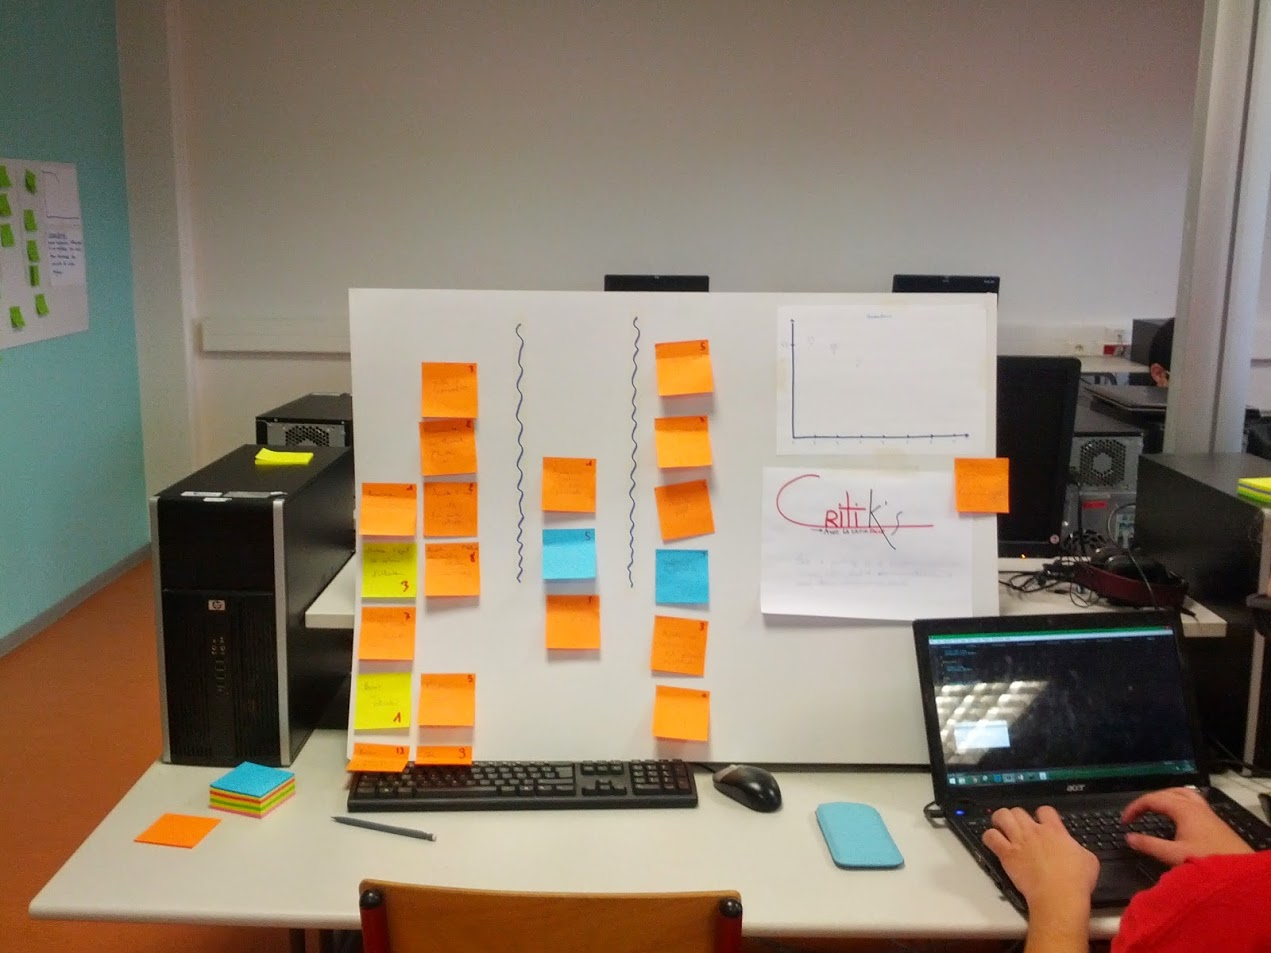
\includegraphics[width=\textwidth]{includes/201410_dashboard.jpg}      
      \end{center}
    \end{column}
    \begin{column}{0.5\textwidth}
      la même recette qu'en S3 avec pour différence : 
      \begin{itemize}
        \item la soutenance se fait sous forme de salon dans une salle de TD
        \item ça se passe en fin de S4
      \end{itemize}
    \end{column}
  \end{columns}
\end{frame}

\subsection{Apprentissages}
\begin{frame}{Octobre 2014 : Apprentissages}
  \begin{itemize}
    \item 1 enseignant pour 26 étudiants c'est très fatiguant mais ça passe,
    \item le salon pour la soutenance c'est jouable,
    \item il manques quelques cours aux étudiants pour être plus autonomes.
  \end{itemize}
\end{frame}

\section{Janvier 2015}
\subsection{Objectifs}
\begin{frame}{Janvier 2015 : Expérience}
  Toute la promo entre la fin du S3 et le début du S4, on vole une semaine de congé.

  Objectifs : 
  \begin{itemize}
    \item valider le passage à l'échelle, 
    \item impliquer des collègues
  \end{itemize}
\end{frame}

\subsection{Déroulement}
\begin{frame}{Janvier 2015 : Déroulement}
  \begin{itemize}
    \item 5 encadrants pour 4 groupes de TP (90 étudiants).
    \item constitution des équipes par les enseignants
    \item 2 équipes issues de la journée entreprenariat
    \item des sujets apportés par les étudiants
    \item les mêmes contraintes technique
  \end{itemize}
\end{frame}

\begin{frame}{Janvier 2015 : Planning}
  \begin{center}
    \begin{tabular}{| c | c | c | c | c |}
      \hline
      \textbf{Jour 1} & \textbf{Jour 2} & \textbf{Jour 3} & \textbf{Jour 4} & \textbf{Jour 5} \\
      \hline \hline
      Lego4scrum      & sprint          & sprint          & sprint          & sprint          \\
      \hline
      backlog         & sprint          & sprint          & sprint          & sprint          \\
      \hline \hline
      sprint 0        & sprint          & sprint          & sprint          & salon           \\
      \hline
      sprint          & sprint          & pitch           & sprint          & rétrospective   \\
      \hline
    \end{tabular}
  \end{center}
\end{frame}

\subsection{Apprentissages}
\begin{frame}{Janvier 2015 : Apprentissages}
  \begin{itemize}
    \item les enseignants non agiliste sont en difficultés techniques
    \item la généralisation est un succès
    \item les étudiants sont enthousiastes
    \item l'activité est trop tôt
    \item ça génère une cohésion de promotion extraordinaire.
  \end{itemize}
\end{frame}

%\begin{frame}{Année 2 (septembre 2014 à juillet 2015)}
%  \begin{itemize}
%    \item de 96h théoriques à XXh pour l'agilité ...
%    \item \textbf{Problématique:} passage à l'échelle
%    \item deuxième expérimentation: large échelle
%      \begin{itemize}
%        \item ensemble de la promotion (90 étudiants)
%        \item besoin d'impliquer des collègues (4 encadrants nécessaires !)
%        \item positionnement entre S3 et S4 (pas l'idéal ... mais le plus "pratique")
%        \item 5 jours du lundi au vendredi, on "vole" une semaine de congés ;)
%        \item 2 équipes issues de la journée entreprenariat sont "protégées"
%        \item un \emph{pitch} investisseurs à mi-parcours, un salon à la fin
%        \item rétrospective \textbf{très très} enthousiaste des étudiants (mais collègues en difficulté)
%      \end{itemize}
%      \item \textbf{Objectif n+1}: mini-projet en début de S3 + projet agile final avant départ en stage !
%  \end{itemize}
%\end{frame}

\section{Octobre 2015}
\subsection{Objectifs}
\subsection{Déroulement}
\begin{frame}{Octobre 2015 : Objectifs}
  \begin{columns}
    \begin{column}{0.5\textwidth}
      \begin{center}
        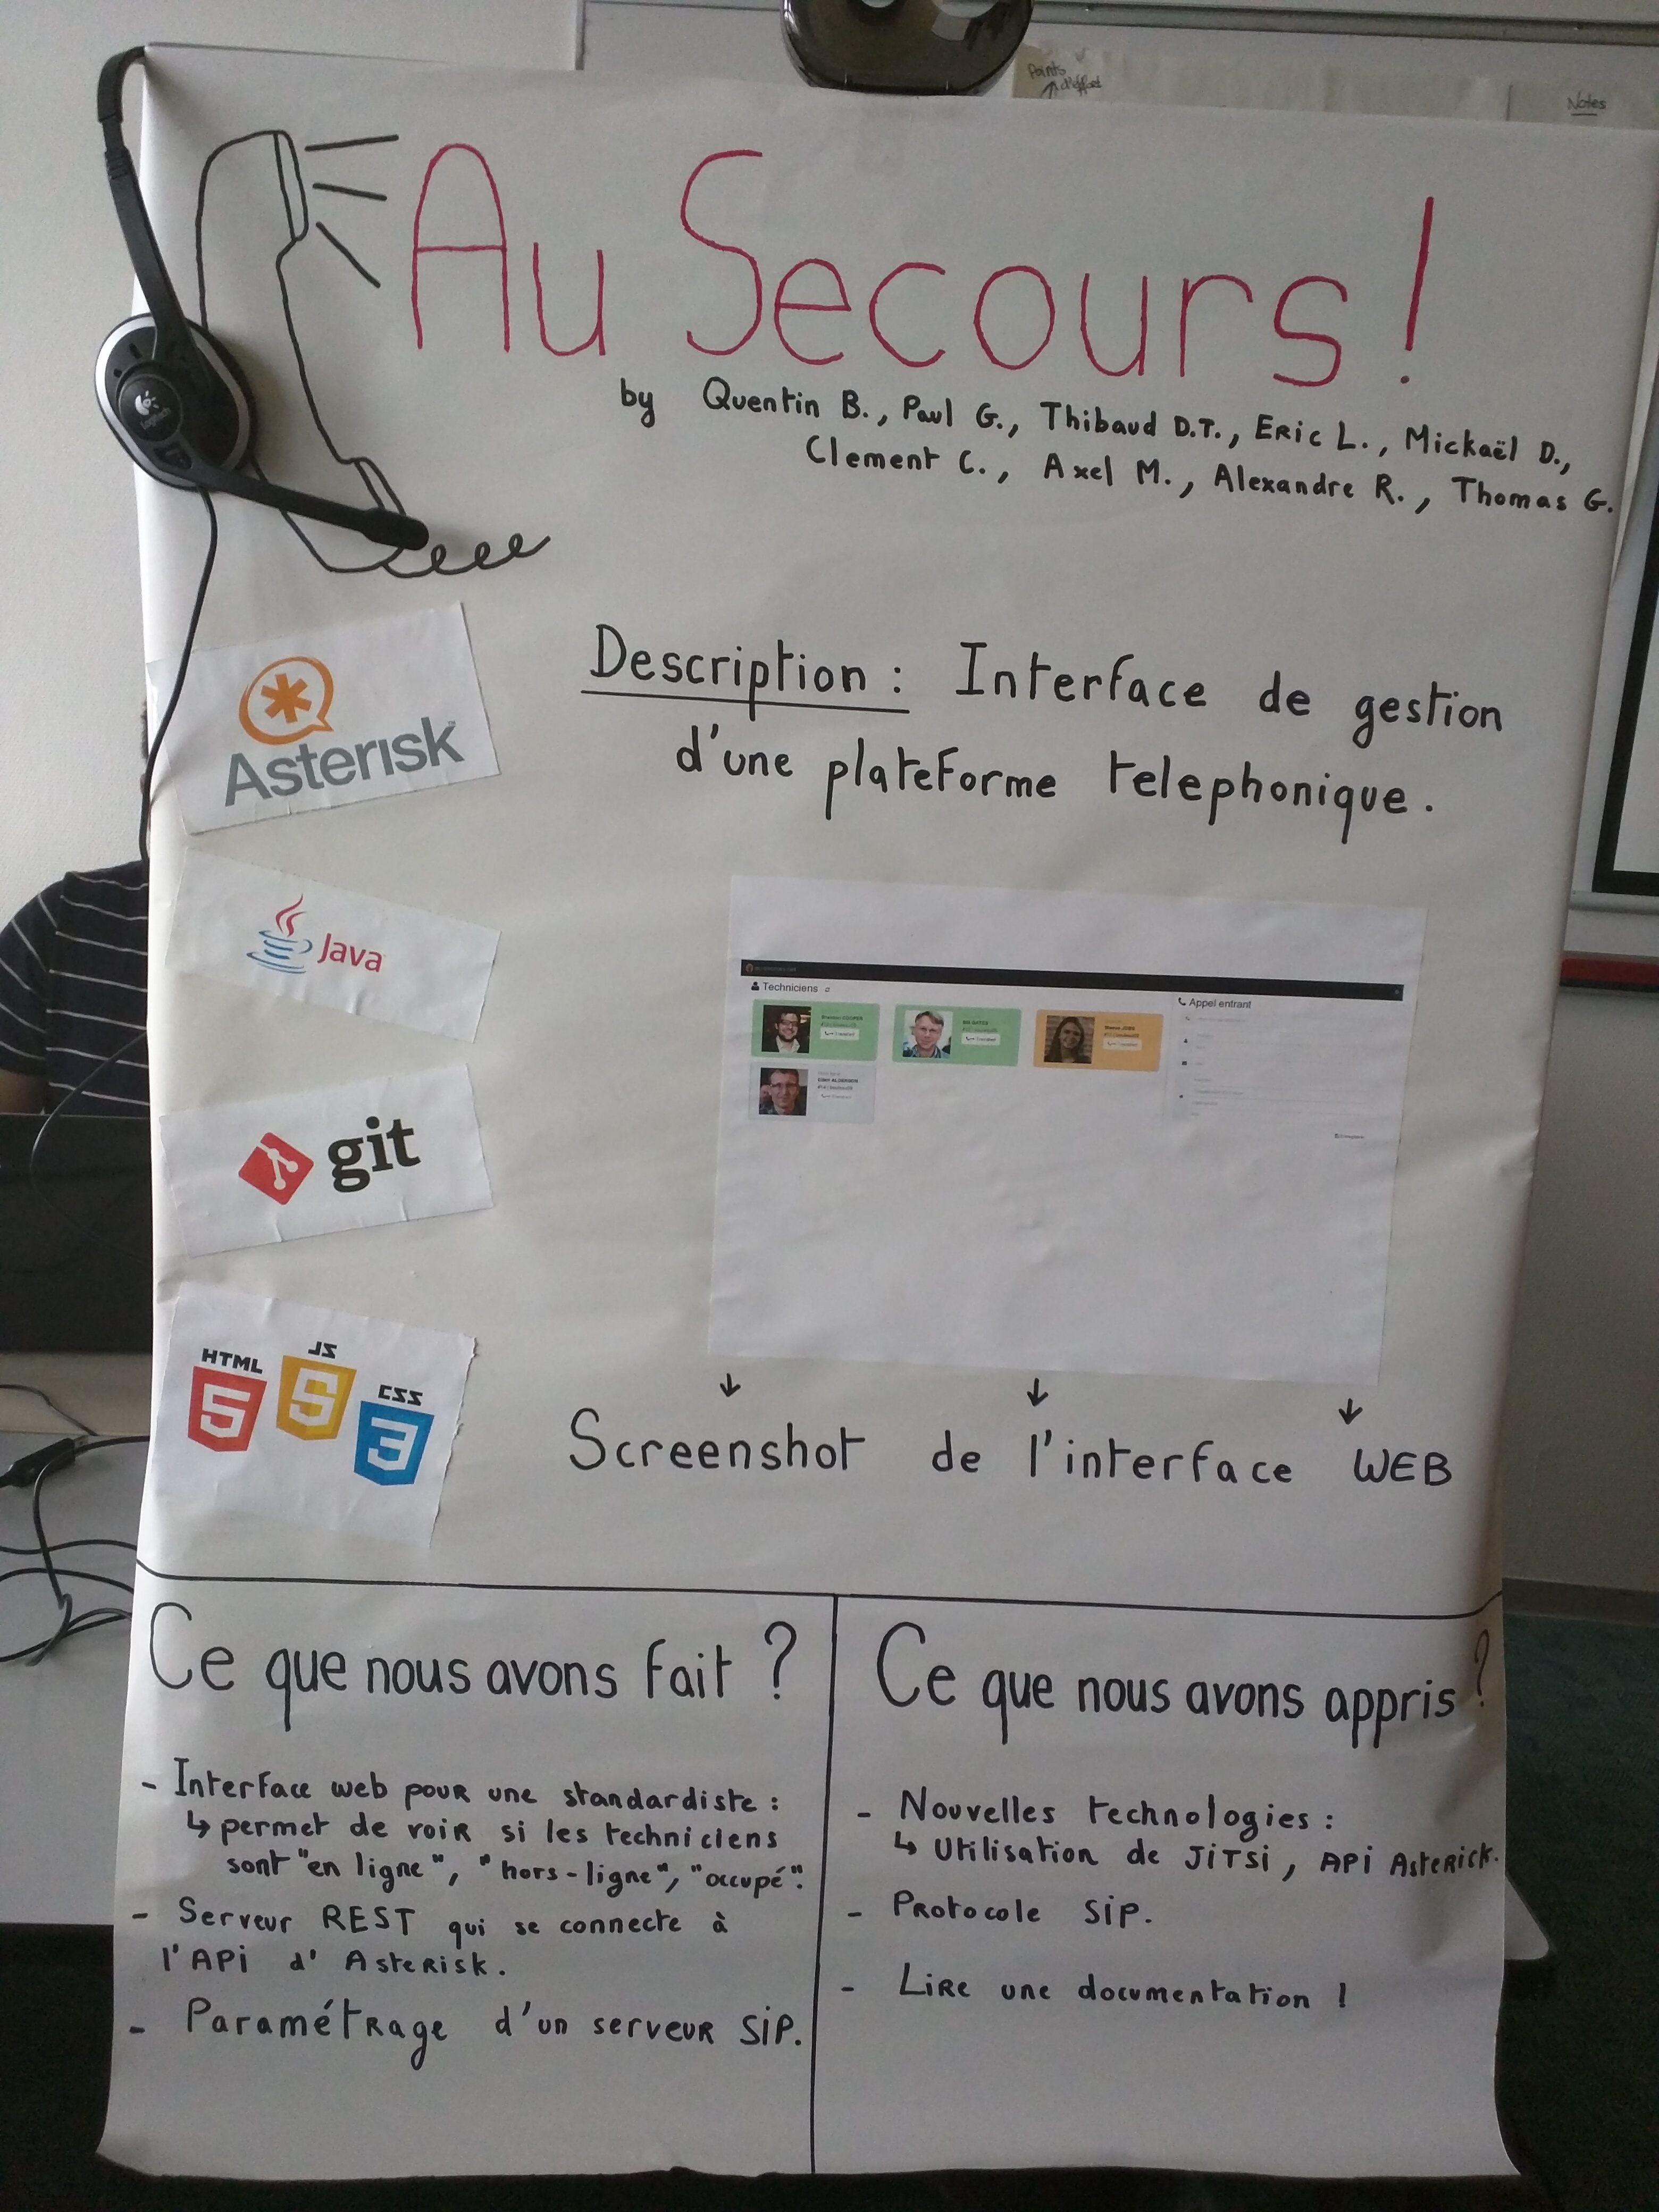
\includegraphics[width=\textwidth]{includes/201510_salon.jpg}      
      \end{center}
    \end{column}
    \begin{column}{0.5\textwidth}
      \begin{itemize}
        \item Objectif : valider la collaboration avec un porteur de projet
        \item Pas d'autres changement.
      \end{itemize}
    \end{column}
  \end{columns}
\end{frame}

\subsection{Apprentissages}
\begin{frame}{Octobre 2014 : Apprentissages}
  \begin{columns}
    \begin{column}{0.5\textwidth}
      \begin{center}
        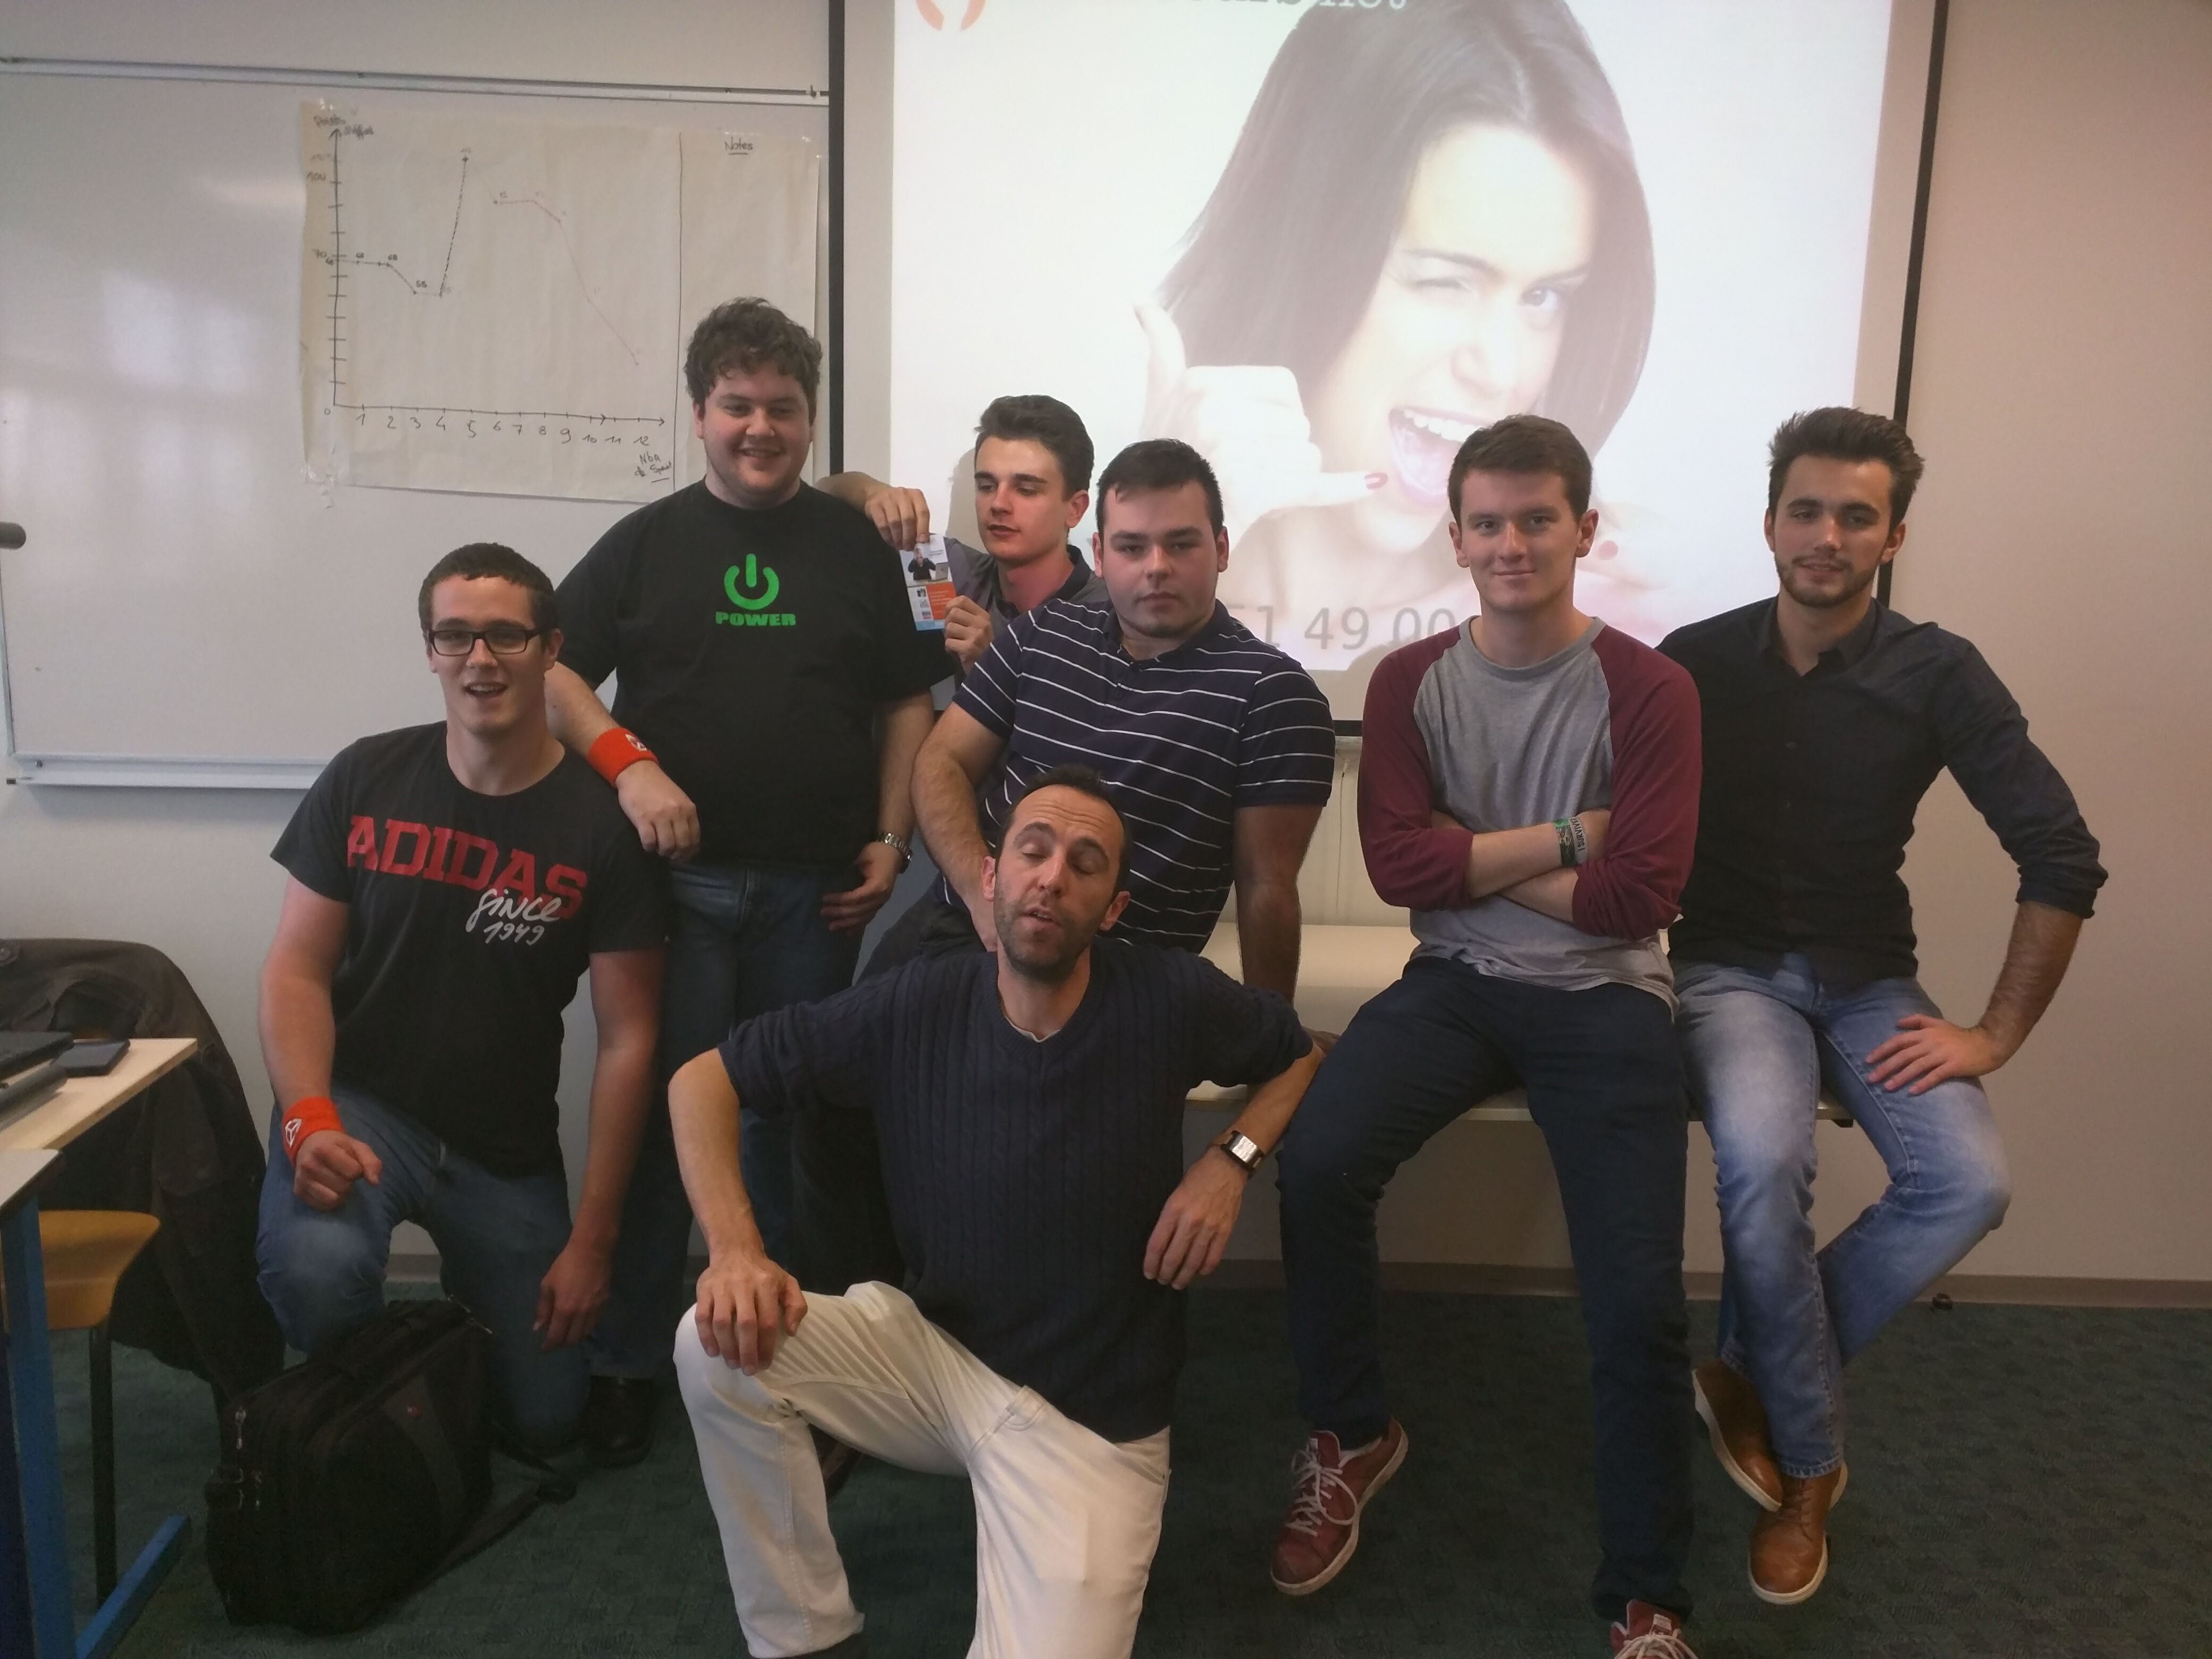
\includegraphics[width=\textwidth]{includes/201510_ausecours.jpg}      
      \end{center}
    \end{column}
    \begin{column}{0.5\textwidth}
  \begin{itemize}
    \item L'intégration du porteur de projet dès les premières minutes est un vrai succès
    \item Le porteur de projet était particulier : amis et technique.
  \end{itemize}
    \end{column}
  \end{columns}
\end{frame}

\begin{frame}{Année 3 (septembre 2015 à juillet 2016)}
  \begin{itemize}
    \item enfin 96h dédiées entièrement à l'agilité :)
    \item \textbf{Problématique:} intégration GEA/INFO + "vrai client" (entrepreneurs) 
    \item troisième expérimentation: l'âge de la maturité ?
      \begin{itemize}
        \item mini-projet agile sur 3j en début de S3
        \begin{itemize}
          \item reboot de POO/COO après les vacances ;)
          \item ensemble de la promotion de S3 (hic: TDD)
          \item collègues de l'année passée poursuivent leur implication :)
          \item un peu trop court, mais première approche
        \end{itemize}
        \item projet agile en S4 décalé
        \begin{itemize}
          \item \emph{comprends pas bien ta phrase ci-dessous: à découper ;)}
          \item Début de S3, S4 décallé avec 1 premier porteur de projet, puis toute la promo à la fin du S4, du mercredi au mercredi avec 6 porteurs de projets et les GEA europe, S3 décallé.
        \end{itemize}
        \item projet agile sur 5j en fin de S4 ...
      \end{itemize}
  \end{itemize}
\end{frame}

\begin{frame}{Année 3 (septembre 2015 à juillet 2016)}
  \begin{itemize}
    \item enfin 96h dédiées entièrement à l'agilité :)
    \item \textbf{Problématique:} intégration GEA/INFO + "vrai client" (entrepreneurs) 
    \item troisième expérimentation: l'âge de la maturité ?
    \begin{itemize}
        \item projet agile sur 5j en fin de S4
        \begin{itemize}
          \item ensemble de la promotion, mais 3 encadrants nécessaire
          \item recrutement d'un agiliste professionnel (plus qu'un naïf dans le coup)
          \item projet arrivant après les cours de REST+JS+Androïd (mieux!)
          \item 5 jours répartis sur 2 semaines (lundi férié, pas de chance)
          \item implication des GEA option "création d'entreprise"
          \item implication de porteur de projets externes: entrepreneurs BGE + Audace
          \item toujours un \emph{pitch} investisseurs à mi-parcours, un salon à la fin
        \end{itemize}
        \item rétrospective \emph{très} enthousiastes des étudiants (effet d'échelle)
      \end{itemize}
      \item \textbf{Objectif n+1}: conserver Laurel (ou Hardy) !
  \end{itemize}
\end{frame}


\begin{frame}{Et maintenant ?}
  \begin{itemize}
    \item Laurel et Hardy, l'aventure continue ?
    \item \'Etape cruciale de la TDD en S3 ...
    \item Renforcement des liens GEA/INFO
      \begin{itemize}
        \item Intégrer les GEA en début de S3 (FI/FC),
        \item équipes communes lors de la journée de l'entreprenariat,
        \item final en beauté avec le projet agile de S4 !
      \end{itemize}
    \item ... et peut-être un jour: DU Lean startup ? :)
  \end{itemize}
\end{frame}

\end{document}

